\documentclass{beamer}

\usepackage{default}
\usepackage{hanging}
\usepackage{amsmath}
\usepackage{amsthm}
\usepackage{amsfonts}
\usepackage{enumerate}

\usetheme{Warsaw}

\usepackage{etoolbox}
\usepackage{xpatch}
\makeatletter
\patchcmd\beamer@@tmpl@frametitle{\insertframetitle}{%
	\ifnumgreater{\arabic{section}}{0}{%
		\thesection.%
		\ifnumgreater{\arabic{subsection}}{0}{% 
			\thesubsection.%
			\ifnumgreater{\arabic{subsubsection}}{0}{%
				\thesubsubsection.%
			}{}%
		}{}%
	}{}%
	~\insertframetitle{}{}%
}%
\makeatother

\setbeamercovered{highly dynamic}
\newcounter{saveenumi}
\newcommand{\seti}{\setcounter{saveenumi}{\value{enumi}}}
\newcommand{\conti}{\setcounter{enumi}{\value{saveenumi}}}
\resetcounteronoverlays{saveenumi}

\usepackage{tikz}
\usetikzlibrary{shapes.geometric, arrows}
\tikzstyle{startstop} = [rectangle, draw, rounded corners, minimum width=3cm, minimum height=1cm, text centered, draw=black]
\tikzstyle{process} = [rectangle, draw, minimum width=3cm, minimum height=1cm, text centered, text width=4cm, draw=black]
\tikzstyle{line} = [draw, -latex']

\newcommand{\R}{\mathbb{R}}

\begin{document}
\title{Progress Report}
\author{Afifah Maya Iknaningrum}
\date{2018}
\institute{Kanazawa University}

\begin{frame}
\titlepage
\end{frame}

\begin{frame}{3D Incompressible Navier-Stokes}
\begin{block}{Strong Form}
	We want to find \[(u,p) : \Omega \times (0,T) \rightarrow \R^3 \times \R\] where $ u $ is unknown velocity and $ p $ is unknown pressure such that
	\begin{equation}\label{Navier-Stokes}
	\begin{cases}
	\dfrac{\partial u}{\partial t} + (u \cdot \nabla) u - \nu \bigtriangleup u + \nabla p = f & \text{ in } \Omega \times (0,T)\\
	\nabla \cdot u = 0 & \text{ in } \Omega \times (0,T)\\
	u = 0 & \text{ on } \partial \Omega \times (0,T)\\
	u = u^0 & \text{ in } \Omega \text{, at } t=0
	\end{cases}
	\end{equation}
	where $ f : \Omega \times (0,T) \rightarrow \R^3 $ and $ u^0 : \Omega \rightarrow \R^3 $ are given functions, choosing $ \nu > 0 , \nu = 1$ is a viscosity.
\end{block}
\end{frame}

\begin{frame}{Incompressible Navier-Stokes}
\begin{block}{Weak Form}
	We want to find $ \{ (u,p)(t) \in V \times Q ; t \in (0.T) \} $ such that for $ t \in (0,T) $
	\begin{equation} \label{NS_Weak} \nonumber
	\begin{cases}
	\big( \dfrac{\partial u}{\partial t} + (u \cdot \nabla)u,v \big) + a(u,v) + b(v,p) + b(u,q) = (f,v) & , \\ \hspace{5cm} \forall(v,q)\in V\times Q \\ u=u^{0} , \hspace{4cm} t=0
	\end{cases}
	\end{equation}
	\begin{eqnarray}\nonumber
	a(u,v) &=& \nu \int_{\Omega} \nabla u : \nabla v \ dx \\ \nonumber
	b(v,q) &=& - \int_{\Omega} (\nabla \cdot v) q \ dx \\ \nonumber
	V &=& H_{0}^{1}(\Omega, \R^d) = H_{0}^{1}(\Omega)^d \\ \nonumber
	Q &=& \{ q\in L^2(\Omega) ; \int_{\Omega} q \ dx=0 \}.
	\end{eqnarray}
\end{block}
\end{frame}

\begin{frame}{3D Discretization}
\begin{block}{First order in time}
	Before applying to FreeFEM++, we need to discritize $ \dfrac{\partial u_{i}}{\partial t} + (u \cdot \nabla)u_{i} $ part, where $ dt $ as time increment.
	\[ \dfrac{\partial u_{i}}{\partial t} + (u \cdot \nabla)u_{i} \approx \dfrac{u_{i}^{n}-u_{i}^{n-1}(X_{1}(u^{n-1},dt))}{dt} + O(dt) \]
\end{block}
\begin{block}{Second order in time / Adam-Bashforth Method}
	\begin{eqnarray}\nonumber
		&\dfrac{\partial u_{i}}{\partial t} + (u \cdot \nabla)u_{i} \approx\\ \nonumber &\dfrac{3u_{i}^{n}-4u_{i}^{n-1}(X_{1}(\tilde{u}^{n-1},dt))+u_{i}^{n-2}(X_{1}(\tilde{u}^{n-1},2dt))}{2\ dt} + O(dt^2)
	\end{eqnarray}
\end{block}
\end{frame}

\begin{frame}
\begin{block}{where}
	\[ X_{1}(u^{n-1},dt)(x) = x - u^{n-1}(x)\ dt\]\\
	\[\tilde{u}^{n-1}_{i} = 2u_{i}^{n-1}-u_{i}^{n-2}\]
\end{block}
\begin{block}{with stabilization term}
	With $ \delta>0 $ and $ h $ as mesh size
	\[ C_{i}(p,q) = \delta \sum_{k} h_{k}^{2}(\nabla p, \nabla q)_{k} \]
\end{block}
\end{frame}

\begin{frame}{Error estimate}
\begin{block}{$ L^{2} $}
	\[\| u_{h}^{n}-u^{n} \|_{\ell^\infty(L^2)} =  max \ \| u_{h}^{n}-u^{n} \|_{L^{2}}\]
	with $ O(h^2) $.
\end{block}
\begin{block}{$ H^{1} $}
	\[\| u_{h}^{n}-u^{n} \|_{\ell^\infty(H^{1})} = max \sqrt{\| u_{h}^{n}-u^{n} \|_{L^2(}^{2} + \| \nabla (u_{h}^{n}-u^{n}) \|_{L^2}^{2}}\]
	with $ O(h) $.
\end{block}
\end{frame}

\begin{frame}{Cubic and Cylindrical domain simulation}
\begin{block}{Exact solution}
		\begin{eqnarray}\nonumber
		u &=& (u_{1},u_{2},u_{3}) \\ \nonumber
		u_{1} &=& -\cos(x_{1}) \sin(x_{2}) \cos(x_3) e^{-2t}\\ \nonumber
		u_{2} &=& \sin(x_{1}) \cos(x_{2}) \cos(x_3) e^{-2t}\\ \nonumber
		u_{3} &=& 0 \\ \nonumber
		p&=& \dfrac{-1}{4} e^{-4t} (\cos(2x_1)+\cos(2x_2)+\cos(2x_3))
		\end{eqnarray}
		such that equation (\ref{Navier-Stokes}) is satisfied with $ f = (f_{1},f_{2},f_3) $. With $ f_{1} = -\cos(x_1) \sin(x_2) \cos(x_3) e^{-2t} $, $ f_{2} = -\sin(x_1) \cos(x_2) \cos(x_3) e^{-2t}  $, and $ f_{3} = -(\dfrac{1}{4})e^{-4t}\sin(2x_3)(2\cos(2x_3)+1)   $
\end{block}
\end{frame}

\begin{frame}
\begin{block}{Error Estimate $ H^{1} $}
	With $ c=\dfrac{\sqrt{2}}{4} $, we choose $ dt = c\sqrt{h} = \dfrac{c}{\sqrt{n}} $ such that
	\[ O(dt^2) + O(h) = O(h) + O(h) = O(h) \]
\end{block}
\begin{block}{Error Estimate $ L^{2} $}
	With $ c=\dfrac{\sqrt{2}}{4} $, we choose $ dt = c\sqrt{h} = \dfrac{c}{\sqrt{n}} $ such that
	\[ O(dt^2) + O(h^2) = O(h) + O(h^2) = O(h) \]
\end{block}
\end{frame}

\begin{frame}
\begin{figure}
	\centering
	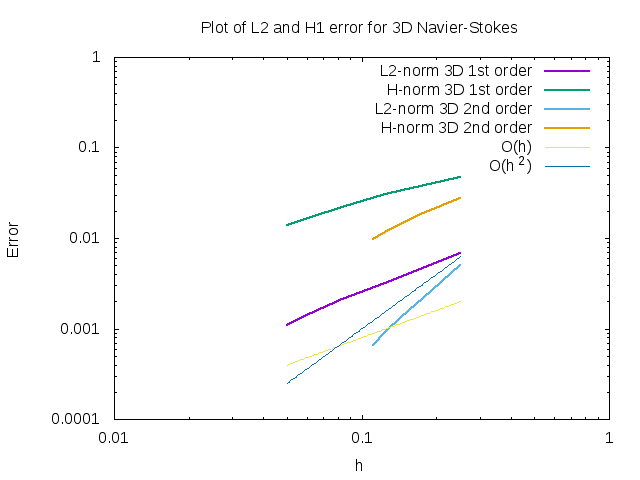
\includegraphics[width=1\linewidth]{NS_3D/error_NS_3D}
	\caption{}
	\label{fig:errorns3d}
\end{figure}
\end{frame}

\begin{frame}
Using the first order in time for the first iteration, and then second order in time for the rest, we obtain :
\begin{figure}
	\centering
	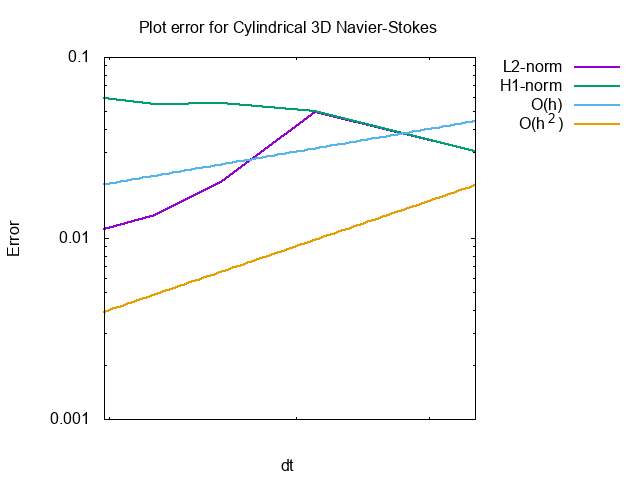
\includegraphics[width=0.8\linewidth]{NS_3D/error_cyl}
	\caption{}
	\label{fig:errorcyl}
\end{figure}
\end{frame}

\begin{frame}
\begin{figure}
	\centering
	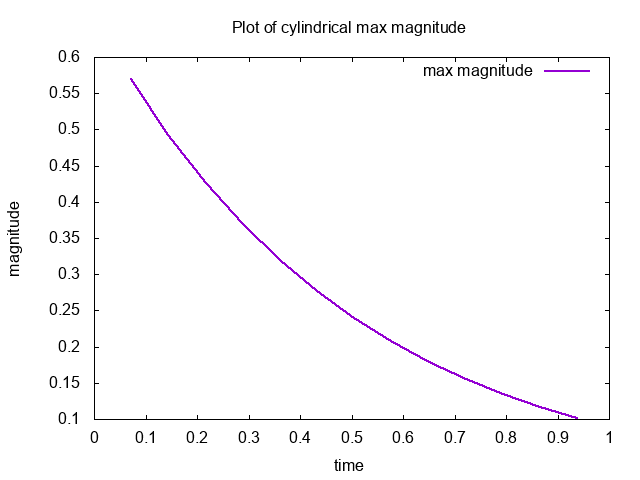
\includegraphics[width=0.9\linewidth]{NS_3D/magnitude_cyl}
	\caption{}
	\label{fig:magnitudecyl}
\end{figure}
\end{frame}

\begin{frame}{Other trial on exact}
\begin{block}{Exact solution}
	with $ c = 8\sqrt{3}/27\pi $
	\begin{eqnarray}\nonumber
	u1 &=& c\sin(\pi x)\sin^2(\pi y)\sin^2(\pi z)\sin(\pi(y+z+t)) \\ \nonumber
	u2 &=& c\sin^2(\pi x)\sin(\pi y)\sin^2(\pi z)\sin(\pi(x+z+t)) \\ \nonumber
	u1 &=& c\sin^2(\pi x)\sin^2(\pi y)\sin(\pi z)\sin(\pi(x+y+t))\\ \nonumber
	p &=& \sin(\pi(x+y+z+t))
	\end{eqnarray}
\end{block}
\end{frame}

\begin{frame}
Such that, for the cylindrical domain, we obtain the error
\begin{figure}
	\centering
	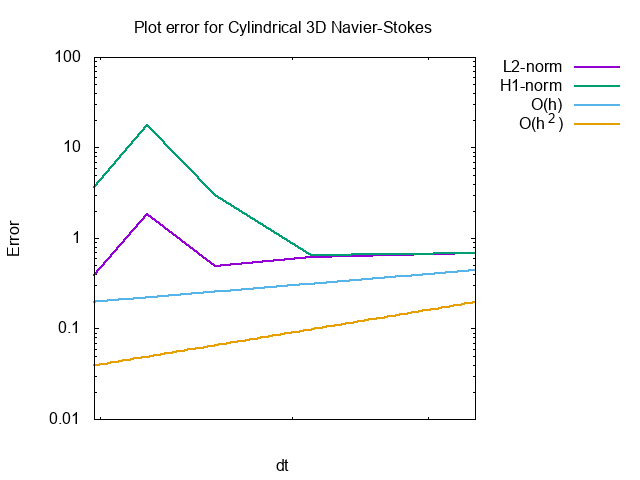
\includegraphics[width=1\linewidth]{NS_3D/error_cyl_2}
	\caption{}
	\label{fig:errorcyl2}
\end{figure}

\end{frame}

\begin{frame}{Tornado simulation on cylindrical domain}
	\begin{block}{Domain and initial condition}
		Taking $ a=1/8, \epsilon_{i} =1, \beta_{i}=1 \ (i=1,\dots,6) $, with domain $ \Omega = \{ x=(x,y,z) \in \R^3 ; -a\leq z\leq 4a, \ \sqrt{x^2+y^2}<1 \} $ and $ u=0 $ on boundary.
		\begin{equation}\label{initial}
		\begin{cases}
		\psi(a,\epsilon,\sigma) &= (a^{2}+\epsilon)^{\sigma}\\
		u_{z} &= \psi(r,\epsilon_{1},-\beta_{1})\psi(z,\epsilon_{2},-\beta_{2})\\ 
		\rho &= \psi(r,\epsilon_{3},-\beta_{3})\psi(z,\epsilon_{4},\beta_{4})\\ 
		u_{0} &= \psi(r,\epsilon_{5},-\beta_{5})\psi(z,\epsilon_{6},-\beta_{6}) \text{\hspace{0.5cm} (with swirl)}\\
		u_{0} &= 0 \text{ \hspace{4cm}(no swirl) }\\
		u_{r} &= sign(z)\rho u_{z}
		\end{cases}
		\end{equation}
	\end{block}
\end{frame}

\begin{frame}{Tornado simulation on cylindrical and curved cylindrical domain}
\begin{block}{Exact solution}
	\begin{eqnarray}\nonumber
	u &=& (u_{1},u_{2},u_{3}) \\ \nonumber
	u_{1} &=& -\cos(x_{1}) \sin(x_{2}) e^{-2t}\\ \nonumber
	u_{2} &=& \sin(x_{1}) \cos(x_{2}) e^{-2t}\\ \nonumber
	u_{3} &=& 0 \\ \nonumber
	p&=& \dfrac{-1}{4} e^{-4t} (\cos(2x_1)+\cos(2x_2))
	\end{eqnarray}
	such that equation (\ref{Navier-Stokes}) is satisfied with $ f = (f_{1},f_{2},f_3) $. With $ f_{1} =0 $, $ f_{2} = 0  $, and $ f_{3} = 0  $. Taking $ \nu=2/3 $ which satisfy the strong formulation
\end{block}
\end{frame}

\begin{frame}
\begin{figure}
	\centering
	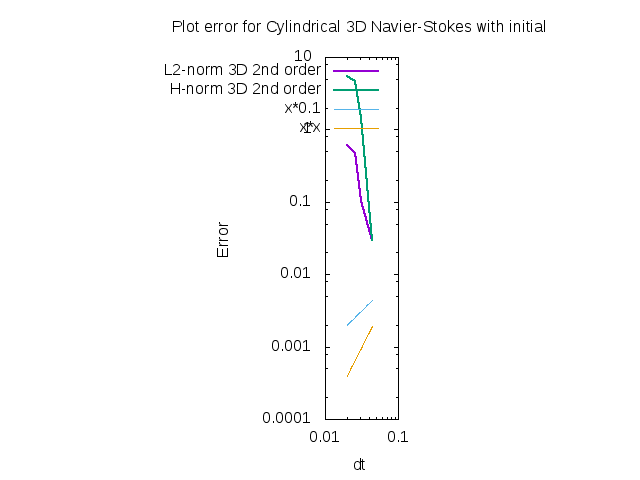
\includegraphics[width=0.9\linewidth]{NS_3D/error_tornado}
	\caption{}
	\label{fig:errortornado}
\end{figure}
\end{frame}

\begin{frame}
\begin{figure}
	\centering
	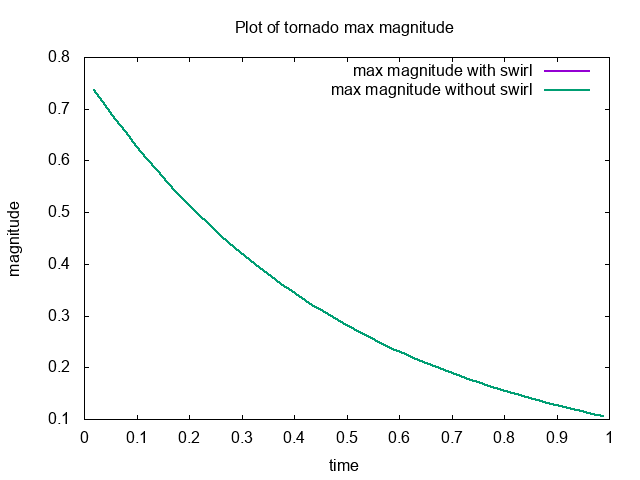
\includegraphics[width=0.9\linewidth]{NS_3D/magnitude_tornado}
	\caption{Max $ v $ of tornado simulation every time step}
	\label{fig:magnitudetornado}
\end{figure}
\end{frame}

\begin{frame}{Tornado simulation on curved cylindrical domain}
Using FreeFEM++ (applying Kazunori's ideas)
\begin{figure}
	\centering
	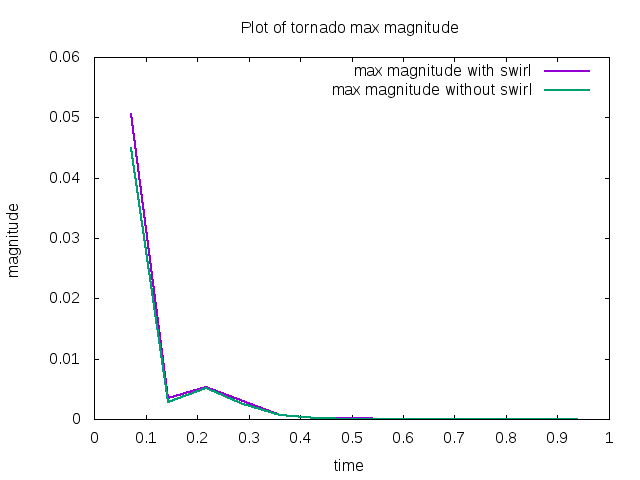
\includegraphics[width=0.9\linewidth]{NS_3D/curved}
	\caption{}
	\label{fig:curved}
\end{figure}
\end{frame}

\begin{frame}
\begin{figure}
	\centering
	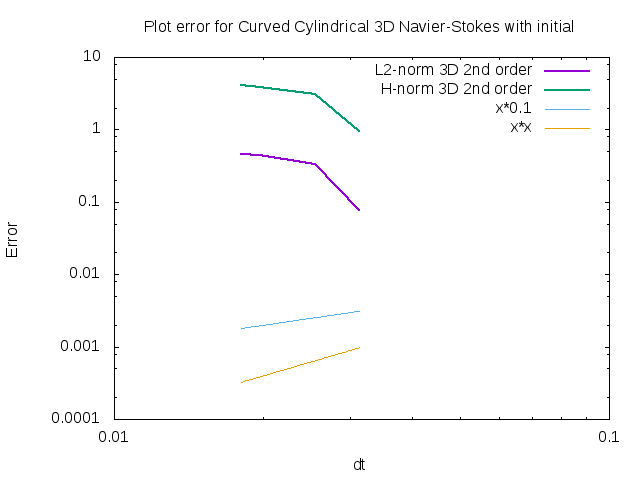
\includegraphics[width=0.9\linewidth]{NS_3D/error_curved}
	\caption{}
	\label{fig:errorcurved}
\end{figure}
\end{frame}

\begin{frame}{Labelling the domain cylinder}
\begin{figure}
	\centering
	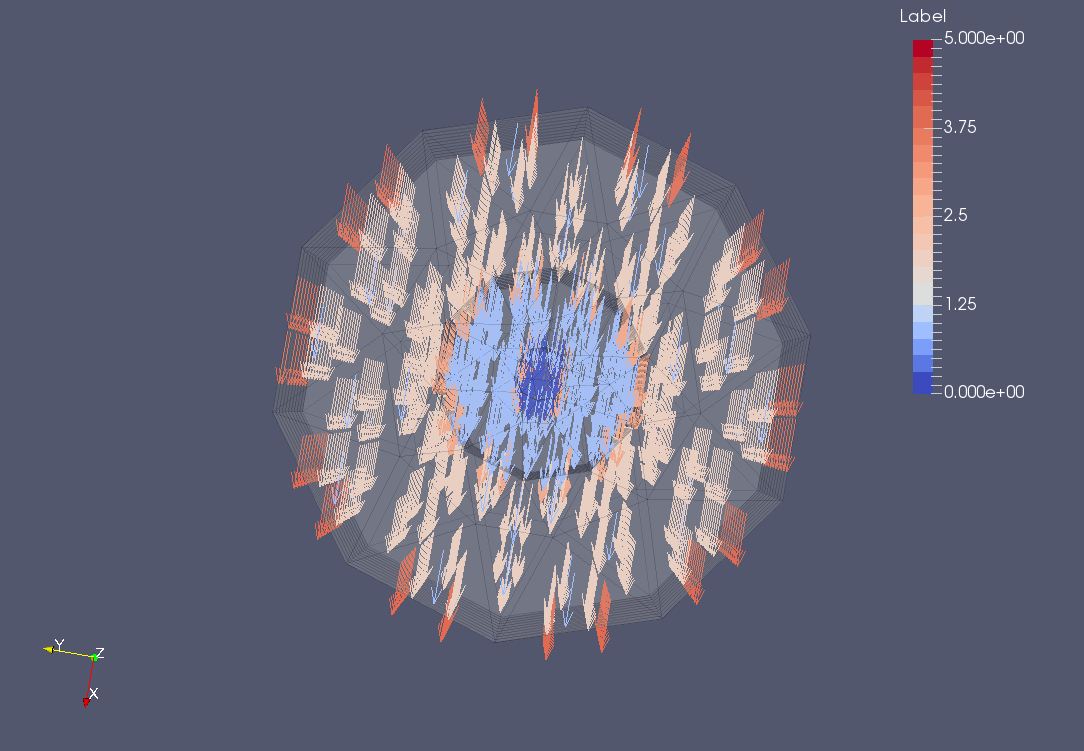
\includegraphics[width=0.7\linewidth]{NS_3D/Label}
	\caption{Labelling}
	\label{fig:label}
\end{figure}
Which is in the program is written as\\
rup=[0,1,1,1,2,1], rdown=[0,1,1,1,2,1], rmid=[1,4,2,3,3,3];
\end{frame}

\begin{frame}{Simulation with initial and Reynolds number}
\begin{block}{Navier-Stokes problem}
	\begin{equation}\nonumber
	\begin{cases}
		\partial_{t} u + (u \cdot \nabla) u - \nu\bigtriangleup u + \nabla p &= 0\\
		u |_{t=0} &=u_{0} \\
		u |_{\partial\Omega} &= 0 \\
		\nabla \cdot u &= 0 \\
	\end{cases}
	\end{equation}
	with the initial in (\ref{initial}). We do the simulation for $ \nu = \dfrac{1}{Re} $, where $ Re = 50000, 10000, 5000, 1000 $. With $ T=5 $, $ h = 1/n = 1/24 $ and $ dt=c\sqrt{h} $ with $ c = \sqrt{2}/8 $.
\end{block}
\end{frame}

\begin{frame}{Cylindrical domain with swirl}
\begin{figure}
	\centering
	\includegraphics[width=1\linewidth]{../../july/Tornado_withswirl}
	\caption{}
	\label{fig:tornadowithswirl}
\end{figure}
\end{frame}

\begin{frame}{Cylindrical domain without swirl}
\begin{figure}
	\centering
	\includegraphics[width=1\linewidth]{../../july/Tornado_noswirl}
	\caption{}
	\label{fig:tornadonoswirl}
\end{figure}

\end{frame}

\begin{frame}{Curved cylindrical domain with swirl}
\begin{figure}
	\centering
	\includegraphics[width=1\linewidth]{../../july/Curved_withswirl}
	\caption{}
	\label{fig:curvedwithswirl}
\end{figure}
\end{frame}

\begin{frame}{Curved cylindrical domain without swirl}
\begin{figure}
	\centering
	\includegraphics[width=1\linewidth]{../../july/Curved_noswirl}
	\caption{}
	\label{fig:curvednoswirl}
\end{figure}

\end{frame}

\end{document}
